\section{MPI-OpenMP Tuning of MUMPS Library}
\label{subseq:mpi-openmp}


As it was mentioned in  section \ref{subseq:mumps-review}, the development of MUMPS began in 1996 when message-passing programming paradigm dominated in parallel computing. Therefore, the library originally was designed only for distributed-memory machines.\\

In 2010,  \citeauthor{chowdhury2010some} published their first experiments and some issues, in \cite{chowdhury2010some}, of exploiting shared memory parallelism in MUMPS. The authors showed that it was possible to achieve some improvements in multicore systems with multithreading, given a purely MPI application. However, later \citeauthor{l2013introduction} mentioned, in \cite{l2013introduction}, that adaptation of existing code for NUMA architecture was still a challenge because of memory allocation, memory affinity, thread pinning and other related issues.\\


In spite of natural data locality of message-passing applications which is always beneficial, a general motivation of switching to a hybrid mode, mixed MPI/OpenMP, is to reduce communication overheads between processes. According to the profiling results done by \citeauthor{chowdhury2010some}, MUMPS contained four main initial sources of shared-memory parallelization, namely: 

\begin{enumerate}

	\item BLAS Level 1, 2, 3 operations during both factorization and solution phases \label{openmp-blocks-1}
	
	\item Assembly operations, where contribution blocks of children nodes of the assembly tree are assembled at the parent level \label{openmp-blocks-2}
	
	\item Copying contribution blocks during stacking operations \label{openmp-blocks-3}
	
	\item Pivot search operations \label{openmp-blocks-4}

\end{enumerate}


Almost all customized BLAS libraries, for example Intel MKL and OpenBLAS, are multi-threaded and can efficiently work in shared-memory environment. Thus, parallelization of region \ref{openmp-blocks-1} can be achieved by linking a suitable BLAS library whereas regions \ref{openmp-blocks-2}, \ref{openmp-blocks-3} and \ref{openmp-blocks-4} are multithreaded by inserting appropriate OpenMP directives above the corresponding loop statements.\\


A detailed review of works \cite{l2013introduction} and \cite{chowdhury2010some} reveals that, in general, a pure OpenMP or mixed MPI/OpenMP strategy can reduce run-time of MUMPS. In average, factorization time is reduced by \textbf{14.3\%} and in some special cases improvement reaches about \textbf{50.4\%}, according to the data provided in the papers. However, at the same time, the results demonstrate that pure-MPI mode sometimes can significantly outperform any hybrid mixed strategy.\\


By and large, the results show two important aspects. Firstly, performance of a specific strategy depends heavily on the resultant assembly tree and thus on the matrix sparsity pattern and applied fill reducing algorithm. Secondly, it is not possible to guess in advance which strategy gives the best parallel performance without detailed information about the tree structure and computational cost per node. \citeauthor{l2013introduction} showed that performance of a particular mode depended on the ratio of large and small fronts. For example, they noticed more threads per MPI process leaded to better parallel performance when the ratio was high. On the other hand, they observed the absolutely opposite result with relatively small ratios. Unfortunately, \citeauthor{l2013introduction} did not provide any quantitative measure for that in their work \cite{l2013introduction}.\\ 


It is also interesting to notice that parallelization of region 1 with using a multithreaded BLAS library brings most of parallel performance for mixed or pure OpenMP strategies, according to the results from\cite{l2013introduction}. But, at the same time, performance of regions 2, 3, 4 multithreaded by OpenMP directives is marginal. In average, it allows to reduce numerical factorization run-time by only \textbf{0.66\%}.\\


This outcome is expected because BLAS subroutines, especially level 3, have a high ratio of floating point operations per memory access and thus PEs re-use data stored in caches as much as possible. Meanwhile, regions 2, 3, 4 mainly perform initialization, data movement and execution of \textit{if-statements} which lead to a low compute ratio.\\


Additionally, it is worth noticing that both works, \cite{chowdhury2010some} and \cite{l2013introduction}, were mainly focused on the numerical factorization phase assuming that both analysis and solution phases do not take lots of time. In spite of credibility of this assumption, it still should be pointed out the solution phase runs faster in case of flat-MPI mode. This fact becomes even more interesting because, in our case, a system with multiple right-hand sides has to be solved in order to generate a preconditioner.\\


We have to admit that both works, \cite{chowdhury2010some} and \cite{l2013introduction}, are relatively old and the analysis above may be not complete and full. Because MUMPS is a dynamic developing project, we can expect that adaptation of shared-memory parallelization in MUMPS has been significantly advanced since that time. Since the release of MUMPS version 4, the developers have persistently recommended to use only a hybrid mode like\textit{one MPI process per socket and as many threads as the number of cores} \cite{mumps-manual}.\\


As an initial test, we decided to compare influence of both Intel MKL and OpenBLAS libraries on parallel performance of MUMPS using GRS matrix set only. In order to pin OpenMP threads in a right way, without any conflict between them, the following OpenMP environment variables were set as:

\begin{itemize}
	\item OMP\_PLACES=cores
	\item OMP\_PROC\_BIND=spread
\end{itemize} 


During the test, we found that run-time of MUMPS-OpenBLAS configuration abnormality increased for some test cases. For instance, in case of matrix \textit{cube-645}, the increase reached almost 450\% in contrast to the pure sequential execution. \\

\figpointer{\ref{fig:mumps-openblas-anomalies}}
\begin{figure}[htpb]
\centering
	\begin{tabular}{cc}
		\subfloat[k3-18]{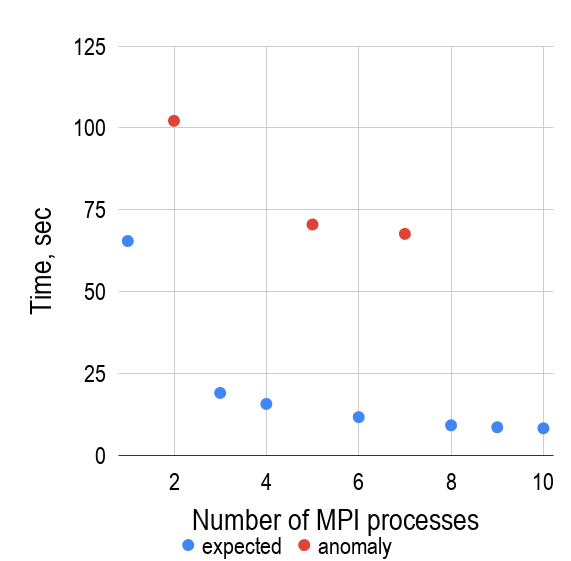
\includegraphics[width=0.4\textwidth]{figures/chapter-2/openmp-mpi/anomalies-k3-18.png}} &
		\subfloat[cube-645]{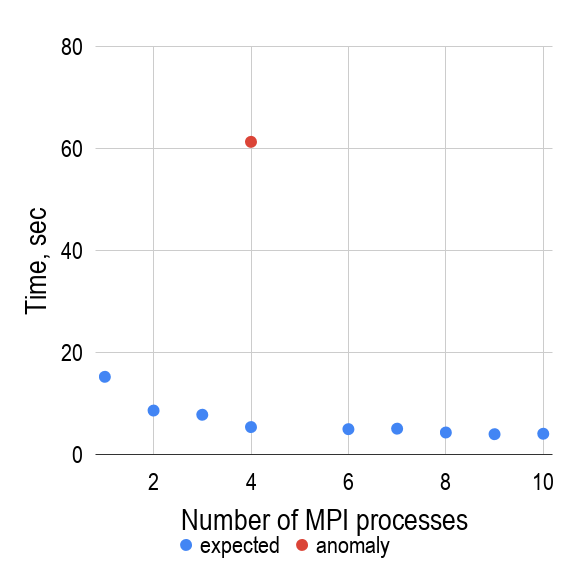
\includegraphics[width=0.4\textwidth]{figures/chapter-2/openmp-mpi/anomalies-cube-645.png}} \\
	\end{tabular}
	\caption{Anomalies of MUMPS-OpenBLAS configuration running with 2 OpenMP threads per MPI process}
	\label{fig:mumps-openblas-anomalies}
\end{figure}


Multiple conflicts between application and system threads were observed using \textit{htop} as an interactive process viewer. Figure \ref{fig:mumps:openblas-thread-conflcit} shows a snapshot taken during factorization of matrix \textit{k3-18} running with 1 MPI process and 20 threads.\\


\figpointer{\ref{fig:mumps:openblas-thread-conflcit}}
\begin{figure}[htpb]
  \centering
  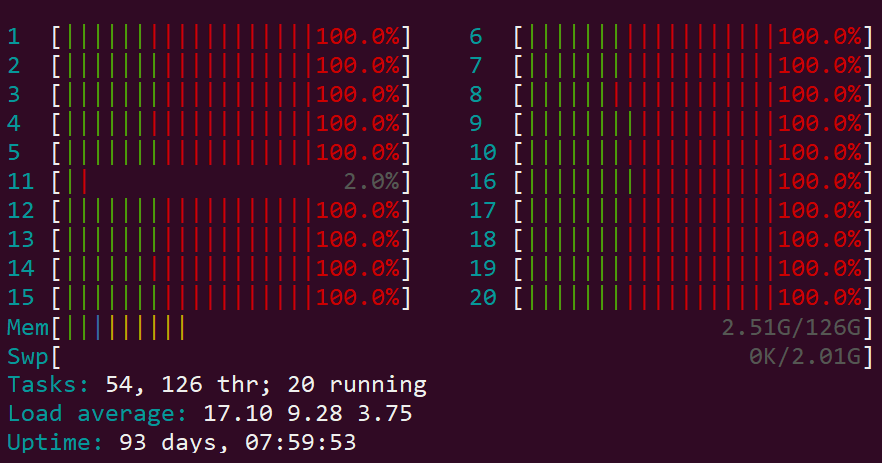
\includegraphics[width=0.75\textwidth]{figures/chapter-2/openmp-mpi/thread-conflict.png}
\caption{A MUMPS-OpenBLAS thread conflict in case of \textit{k3-18} matrix factorization (green - application threads, red - system threads)}
\label{fig:mumps:openblas-thread-conflcit}
\end{figure}


It is difficult to say what exactly caused such behavior. However, \citeauthor{chowdhury2010some} also reported about the same problem with using GotoBLAS (OpenBLAS). They assumed that GotoBLAS created and kept some threads active even after the main threads returned to the calling application which could lead to interference with threads created in other OpenMP regions \cite{chowdhury2010some}. For that reason, we decided to stick only to Intel MKL library for the rest of the study in this section because there were no conflicts detected during initial runs.\\


At the beginning, only common mixed MPI/OpenMP modes were tested in order to check influence of shared-memory parallelism on parallel performance of MUMPS as well as to limit the amount of testing. The following strategies were chosen, namely: 20 MPI - 1 thread (flat-MPI), 10 MPI - 2 threads, 4 MPI - 5 threads, 2 MPI - 10 threads, 1 MPI - 20 threads (flat-OpenMP). Additionally, MUMPS was set as a preconditioning algorithm for the GMRES solver with only \textit{one iteration}. This allowed to force MUMPS library to solve systems multiple right-hand sides. According to our assumption, time spent on one GMRES iteration is negligible in contrast time spent on sparse direct matrix factorization. The test results are shown in tables BRA, BRA and BRA as well as in appendix BRA. Numerical values in tables are given in seconds.\\


%%%%%%%%%%%%%%%%%%%%%%%%%%%%%%%%%%%%%%%%%%%%%%%%%%%%
\begin{table}[h!]
\centering
\begin{tabular}{|c|c|c|c|c|c|c|}
\hline
\begin{tabular}[c]{@{}c@{}}Matrix\\ Name\end{tabular} & \begin{tabular}[c]{@{}c@{}}20 MPI\\ 1 thread\end{tabular} & \begin{tabular}[c]{@{}c@{}}10 MPI\\ 2 threads\end{tabular} & \begin{tabular}[c]{@{}c@{}}4 MPI\\ 5 threads\end{tabular} & \begin{tabular}[c]{@{}c@{}}2 MPI\\ 10 threads\end{tabular} & \begin{tabular}[c]{@{}c@{}}1 MPI\\ 20 threads\end{tabular} & \begin{tabular}[c]{@{}c@{}}Gain\\ w.r.t.\\ flat-MPI\end{tabular} \\ \hline
k3-18                                                 & \textbf{12.520}                                           & 12.630                                                     & 14.010                                                    & 18.020                                                     & 19.170                                                     & -                                                                \\ \hline
k3-2                                                  & 1.341                                                     & \textbf{1.250}                                             & 1.470                                                     & 1.671                                                      & 2.052                                                      & 1.073                                                            \\ \hline
cube-645                                              & \textbf{6.585}                                            & 6.859                                                      & 8.552                                                     & 12.010                                                     & 14.080                                                     & -                                                                \\ \hline
cube-64                                               & 0.756                                                     & \textbf{0.749}                                             & 0.874                                                     & 1.178                                                      & 1.354                                                      & 1.010                                                            \\ \hline
cube-5                                                & 0.181                                                     & 0.132                                                      & \textbf{0.104}                                            & 0.126                                                      & 0.117                                                      & 1.744                                                            \\ \hline
pwr-3d                                                & 0.130                                                     & 0.114                                                      & 0.0972                                                    & \textbf{0.077}                                             & 0.109                                                      & 1.691                                                            \\ \hline
\end{tabular}
\caption{GRS - HW1}
\label{fig:mpi-omp-grs-hw1}
\end{table}



\begin{table}[h!]
\centering
\begin{tabular}{|c|c|c|c|c|c|c|}
\hline
\begin{tabular}[c]{@{}c@{}}Matrix\\ Name\end{tabular} & \begin{tabular}[c]{@{}c@{}}20 MPI\\ 1 thread\end{tabular} & \begin{tabular}[c]{@{}c@{}}10 MPI\\ 2 threads\end{tabular} & \begin{tabular}[c]{@{}c@{}}4 MPI\\ 5 threads\end{tabular} & \begin{tabular}[c]{@{}c@{}}2 MPI\\ 10 threads\end{tabular} & \begin{tabular}[c]{@{}c@{}}1 MPI\\ 20 threads\end{tabular} & \begin{tabular}[c]{@{}c@{}}Gain\\ w.r.t.\\ flat-MPI\end{tabular} \\ \hline
k3-18                                                 & 8.558                                                     & \textbf{7.819}                                             & 8.165                                                     & 11.330                                                     & 14.320                                                     & 1.095                                                            \\ \hline
k3-2                                                  & 1.168                                                     & \textbf{0.788}                                             & 0.956                                                     & 1.131                                                      & 1.651                                                      & 1.482                                                            \\ \hline
cube-645                                              & 5.735                                                     & \textbf{4.859}                                             & 6.069                                                     & 9.360                                                      & 11.040                                                     & 1.180                                                            \\ \hline
cube-64                                               & 0.805                                                     & \textbf{0.541}                                             & 0.664                                                     & 0.947                                                      & 0.918                                                      & 1.490                                                            \\ \hline
cube-5                                                & 0.241                                                     & 0.121                                                      & \textbf{0.093}                                            & 0.129                                                      & 0.126                                                      & 2.582                                                            \\ \hline
pwr-3d                                                & 0.234                                                     & 0.095                                                      & 0.098                                                     & \textbf{0.070}                                             & 0.094                                                      & 3.341                                                            \\ \hline
\end{tabular}
\caption{GRS - HW2}
\label{fig:mpi-omp-grs-hw2}
\end{table}


%%%%%%%%%%%%%%%%%%%%%%%%%%%%%%%%%%%%%%%%%%%%%%%%%%%%
\begin{table}[h!]
\centering
\begin{tabular}{|c|c|c|c|c|c|c|}
\hline
\begin{tabular}[c]{@{}c@{}}Matrix\\ Name\end{tabular} & \begin{tabular}[c]{@{}c@{}}20 MPI\\ 1 thread\end{tabular} & \begin{tabular}[c]{@{}c@{}}10 MPI\\ 2 threads\end{tabular} & \begin{tabular}[c]{@{}c@{}}4 MPI\\ 5 threads\end{tabular} & \begin{tabular}[c]{@{}c@{}}2 MPI\\ 10 threads\end{tabular} & \begin{tabular}[c]{@{}c@{}}1 MPI\\ 20 threads\end{tabular} & \begin{tabular}[c]{@{}c@{}}Gain\\ w.r.t.\\ flat-MPI\end{tabular} \\ \hline
cant                                                  & 1.400                                                     & \textbf{0.990}                                             & 1.050                                                     & 1.605                                                      & 2.019                                                      & 1.414                                                            \\ \hline
consph                                                & 3.495                                                     & \textbf{2.652}                                             & 3.015                                                     & 3.706                                                      & 3.714                                                      & 1.318                                                            \\ \hline
memchip                                               & \textbf{7.470}                                            & 9.080                                                      & 13.301                                                    & 20.198                                                     & 45.800                                                     & -                                                                \\ \hline
PFlow\_742                                            & 26.802                                                    & 24.204                                                     & \textbf{21.897}                                           & 30.389                                                     & 54.501                                                     & 1.224                                                            \\ \hline
pkustk10                                              & \textbf{0.748}                                            & 0.879                                                      & 0.972                                                     & 1.459                                                      & 1.280                                                      & -                                                                \\ \hline
torso3                                                & \textbf{3.922}                                            & 4.285                                                      & 4.642                                                     & 5.603                                                      & 8.144                                                      & -                                                                \\ \hline
x104                                                  & \textbf{1.597}                                            & 1.644                                                      & 2.024                                                     & 3.208                                                      & 2.167                                                      & -                                                                \\ \hline
CurlCurl\_3                                           & 49.250                                                    & 44.120                                                     & \textbf{39.909}                                           & 43.311                                                     & 63.001                                                     & 1.234                                                            \\ \hline
Geo\_1438                                             & 478.101                                                   & 234.697                                                    & \textbf{151.603}                                          & 157.697                                                    & 158.102                                                    & 3.154                                                            \\ \hline
\end{tabular}
\caption{SuiteSparse - HW1}
\label{fig:mpi-omp-suitesparse-hw1}
\end{table}




\begin{table}[h!]
\centering
\begin{tabular}{|c|c|c|c|c|c|c|}
\hline
\begin{tabular}[c]{@{}c@{}}Matrix\\ Name\end{tabular} & \begin{tabular}[c]{@{}c@{}}20 MPI\\ 1 thread\end{tabular} & \begin{tabular}[c]{@{}c@{}}10 MPI\\ 2 threads\end{tabular} & \begin{tabular}[c]{@{}c@{}}4 MPI\\ 5 threads\end{tabular} & \begin{tabular}[c]{@{}c@{}}2 MPI\\ 10 threads\end{tabular} & \begin{tabular}[c]{@{}c@{}}1 MPI\\ 20 threads\end{tabular} & \begin{tabular}[c]{@{}c@{}}Gain\\ w.r.t\\ flat-MPI\end{tabular} \\ \hline
cant                                                  & 2.128                                                     & \textbf{0.955}                                             & 1.011                                                     & 1.577                                                      & 2.058                                                      & 2.229                                                           \\ \hline
consph                                                & 3.840                                                     & \textbf{2.852}                                             & 3.111                                                     & 3.695                                                      & 3.897                                                      & 1.346                                                           \\ \hline
memchip                                               & \textbf{7.811}                                            & 7.816                                                      & 9.811                                                     & 15.160                                                     & 31.969                                                     & -
\\ \hline
PFlow\_742                                            & 24.190                                                    & 29.241                                                     & \textbf{19.686}                                           & 27.530                                                     & 55.431                                                     & 1.230                                                           \\ \hline
pkustk10                                              & 1.373                                                     & \textbf{0.904}                                             & 1.022                                                     & 1.421                                                      & 1.403                                                      & 1.520                                                           \\ \hline
torso3                                                & 4.733                                                     & \textbf{4.080}                                             & 4.483                                                     & 5.648                                                      & 8.217                                                      & 1.160                                                           \\ \hline
x104                                                  & 2.676                                                     & \textbf{1.597}                                             & 2.025                                                     & 3.204                                                      & 2.133                                                      & 1.676                                                           \\ \hline
CurlCurl\_3                                           & 39.890                                                    & \textbf{34.579}                                            & 38.620                                                    & 41.171                                                     & 67.760                                                     & 1.154                                                           \\ \hline
Geo\_1438                                             & xxx                                                       & yyy                                                        & zzz                                                       & aaa                                                        & bbb                                                        & ccc                                                             \\ \hline
\end{tabular}
\caption{SuiteSparse - HW2}
\label{fig:mpi-omp-suitesparse-hw2}
\end{table}

% mention their hardware


% mention about the PETSc experement with GRS matrices. They reproduced our result


% say that the results are relatively old and maybe there is no sense to trust them




% show a result where multithreding works
